\section{Διαδίκτυο των Πραγμάτων}
\label{sec:iot}
Το \textbf{Διαδίκτυο των Πραγμάτων} (μτφ. \textbf{Internet of Things}, εν συντομία \textbf{ΙοΤ}) είναι ένα σύνολο φυσικών αντικειμένων τα οποία έχουν αισθητήρες, λογισμικό, υπολογιστική ισχύ κτλ. και τα οποία ανταλλάσσουν δεδομένα μεταξύ τους μέσω του Διαδικτύου ή ενός οποιουδήποτε άλλου δικτύου επικοινωνίας. Τα αντικείμενα αυτά μπορεί να είναι ένας άνθρωπος με βηματοδότη στην καρδιά, ένα έξυπνο ρολόι που μετράει παλμούς, ένας καθρέφτης που διαβάζει δεδομένα από αισθητήρες και εμφανίζει πληροφορίες για την κατάσταση του χρήστη.

\subsection{Πώς δουλεύει το ΙοΤ}
Ένα σύστημα ΙοΤ περιέχει πολλές φυσικές μονάδες (hardware) οι οποίες μπορούν να χωριστούν στις ακόλουθες κατηγορίες {\cite{chebudie}}:
\begin{itemize}
    \item Αισθητήρες \& Ενεργοποιητές (Sensors \& Actuators)
    \item Μονάδες Επεξεργασίας (Processing Units)
    \item Μονάδες Αποθήκευσης (Storage Units)
    \item Μονάδες Επικοινωνίας (Communication Units)
\end{itemize}

Σε ό,τι αφορά το λογισμικό των ΙοΤ συσκευών, δεν υπάρχει κάποια συγκεκριμένη αρχιτεκτονική που να ακολουθείται καθολικά. Έχουν προταθεί αρκετές, ενώ παρακάτω παρουσιάζονται 2 από τις πιο διαδεδομένες, η αρχιτεκτονική 3 επιπέδων και η αρχιτεκτονική 5 επιπέδων \cite{sethi}.

\subsubsection{Αρχιτεκτονική 3 επιπέδων}
Η αρχιτεκτονική 3 επιπέδων είναι από τις πιο βασικές και πρώιμες αρχιτεκτονικές που αναπτύχθηκαν και απεικονίζεται στο Σχήμα \ref{fig:iot_3_tier}.
\begin{figure}[h]
    \centering
    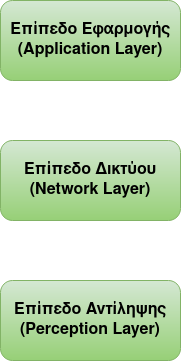
\includegraphics[scale=0.7]{images/chapter2/IoT_3tier.png}
    \caption{Αρχιτεκτονική 3 Επιπέδων}
    \label{fig:iot_3_tier}
\end{figure}

Όπως προκύπτει και από το όνομα αποτελείται από 3 επίπεδα:
\begin{itemize}
    \item \textbf{Επίπεδο Αντίληψης:} Το επίπεδο αντίληψης είναι το φυσικό επίπεδο (hardware) το οποίο περιέχει αισθητήρες για λήψη πληροφοριών και ανίχνευση παραμέτρων από τον περιβάλλοντα χώρο.
    \item \textbf{Επίπεδο Δικτύου:} Το επίπεδο δικτύου είναι υπεύθυνο για την διασύνδεση με άλλες συσκευές, έξυπνα πράγματα κτλ. Χρησιμοποιείται επίσης για την μετάδοση και επεξεργασία δεδομένων των αισθητήρων.
    \item \textbf{Επίπεδο Εφαρμογής:} Το επίπεδο εφαρμογής είναι υπεύθυνο για την παροχή υπηρεσιών συγκεκριμένης εφαρμογής (application specific services) στον χρήστη. Καθορίζει τις διάφορες εφαρμογές στις οποίες μπορεί να αναπτυχθεί το ΙοΤ, όπως το έξυπνο σπίτι, ο έξυπνος καθρέφτης κ.α.
\end{itemize}

\subsubsection{Αρχιτεκτονική 5 επιπέδων}
Η αρχιτεκτονική των 3 επιπέδων περιγράφει την βασική ιδέα πίσω από το ΙοΤ, αλλά στην πράξη δεν επαρκή. Για το λόγο αυτό, υπάρχουν αρχιτεκτονικές με περισσότερα επίπεδα στην βιβλιογραφία. Μία από αυτές είναι η αρχιτεκτονική 5 επιπέδων που φαίνεται στο Σχήμα \ref{fig:iot_5_tier}.

\begin{figure}[h]
    \centering
    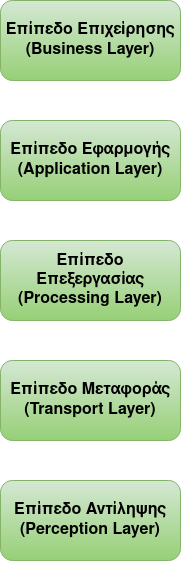
\includegraphics[scale=0.7]{images/chapter2/IoT_5tier.png}
    \caption{Αρχιτεκτονική 5 Επιπέδων}
    \label{fig:iot_5_tier}
\end{figure}

Στην περίπτωση αυτή, τα επίπεδα Αντίληψης και Εφαρμογής παραμένουν ίδια με αυτά της αρχιτεκτονικής 3 επιπέδων ενώ επεξηγούνται και τα υπόλοιπα 3 επίπεδα:
\begin{itemize}
    \item \textbf{Επίπεδο Μεταφοράς:} Το επίπεδο μεταφοράς, μεταδίδει τα δεδομένα των αισθητήρων από το επίπεδο αντίληψης στο επίπεδο επεξεργασίας και αντίστροφα μέσω δικτύων όπως 3G, LAN, RFID, NFC κτλ.
    \item \textbf{Επίπεδο Επεξεργασίας:} Το επίπεδο επεξεργασίας, γνωστό και ως middleware, αποθηκεύει, αναλύει και επεξεργάζεται μεγάλο όγκο δεδομένων που προέρχονται από το επίπεδο μεταφοράς. Προσφέρει μια ευρεία γκάμα υπηρεσιών στα χαμηλότερα επίπεδα. Χρησιμοποιεί επίσης πολλές τεχνολογίες όπως βάσεις δεδομένων, υπολογιστική νέφους και ενότητες επεξεργασίας μεγάλων δεδομένων.
    \item \textbf{Επίπεδο Επιχείρησης:} Το επίπεδο επιχείρησης διαχειρίζεται όλο το ΙοΤ σύστημα, συμπεριλαμβανομένων των εφαρμογών του, των επιχειρηματικών του μοντέλων και της ιδιωτικότητας των χρηστών.
\end{itemize}